% Adapted from haiyichen001/tikz-figure-skill transformer.tex
% Revision 5952e18631600aa46de91ea7653f92ae6697d774; see adjacent MIT license.
% Changes: explicit embeddings, Q/K/V ownership, directed edges, compact post-norm topology.
\documentclass[tikz,border=10pt]{standalone}
\usepackage{amsmath,amssymb}
\usetikzlibrary{positioning,fit,arrows.meta,calc,backgrounds}
\definecolor{acaBlueLine}{HTML}{6080B0}
\definecolor{acaBlueFill}{HTML}{DBEAFE}
\definecolor{acaGreenLine}{HTML}{308568}
\definecolor{acaGreenFill}{HTML}{D7EBDF}
\definecolor{acaOrangeLine}{HTML}{B87930}
\definecolor{acaOrangeFill}{HTML}{FFE6CC}
\definecolor{acaPurpleLine}{HTML}{87639C}
\definecolor{acaPurpleFill}{HTML}{EDE3F2}
\definecolor{acaGreyLine}{HTML}{666666}
\definecolor{acaGreyFill}{HTML}{F5F5F5}
% Edit labels, layer counts, and spacing here. Keep Q and K,V sources unchanged.
\def\encCount{N_e}\def\decCount{N_d}\def\colSep{6.6}
\pgfmathsetmacro{\decBypass}{\colSep+2.2}
\pgfmathsetmacro{\memoryLane}{\colSep/2}
\def\boxWidth{3.4cm}\def\encInput{Source tokens}
\def\decInput{Shifted target tokens}
\begin{document}
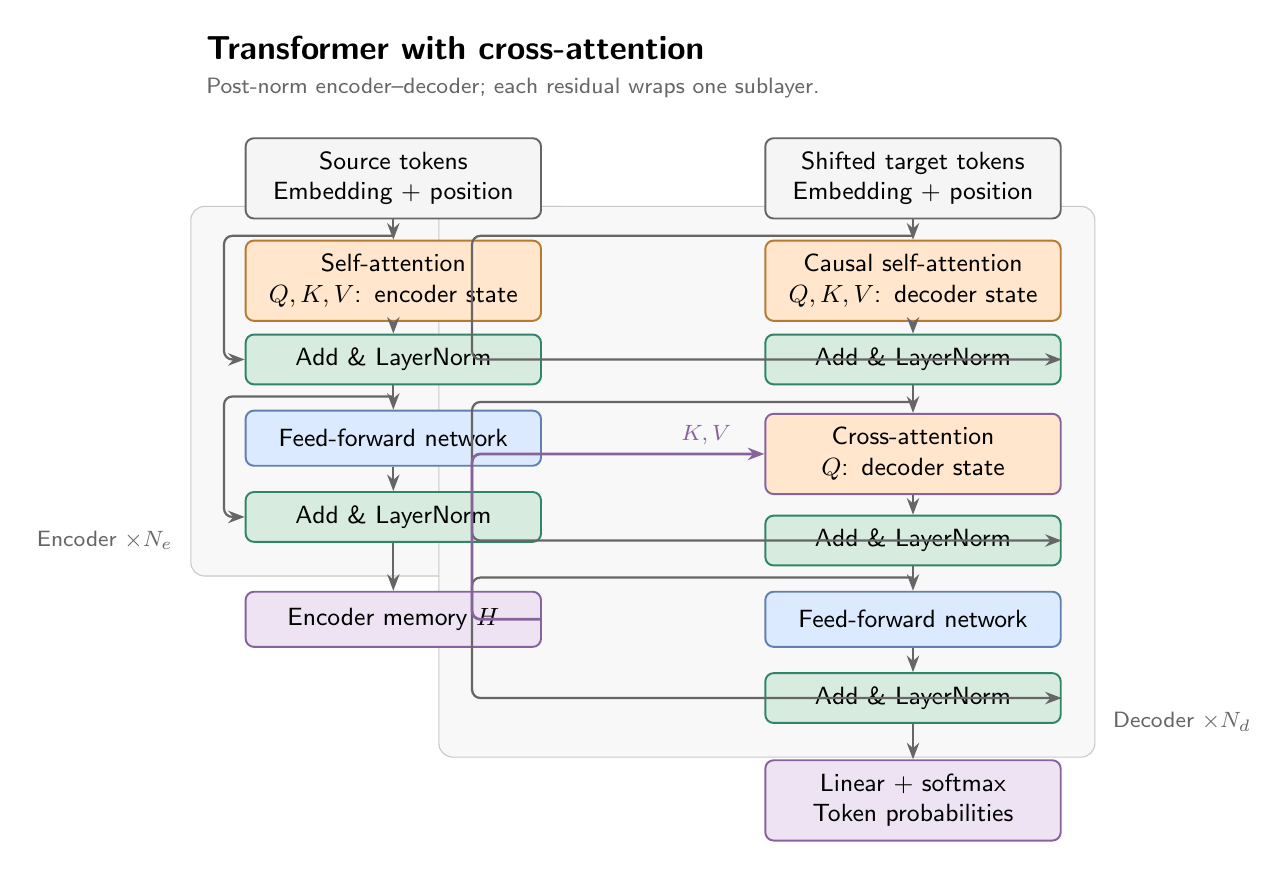
\begin{tikzpicture}[
 >={Stealth[length=2.1mm]},font=\sffamily\small,
 layer/.style={draw=acaGreyLine,fill=white,rounded corners=3pt,align=center,
 text width=\boxWidth,minimum height=.70cm,inner sep=5pt,line width=.7pt},
 attn/.style={layer,fill=acaOrangeFill,draw=acaOrangeLine},
 norm/.style={layer,fill=acaGreenFill,draw=acaGreenLine,minimum height=.52cm},
 ffn/.style={layer,fill=acaBlueFill,draw=acaBlueLine},
 io/.style={layer,fill=acaGreyFill},
 flow/.style={->,draw=acaGreyLine,line width=.8pt},
 residual/.style={flow,rounded corners=3pt},
 context/.style={->,draw=acaPurpleLine,line width=1pt,rounded corners=3pt},
 stack/.style={draw=acaGreyLine!35,fill=acaGreyFill!70,rounded corners=5pt,inner sep=12pt},
 smalllabel/.style={font=\sffamily\footnotesize,text=acaGreyLine}]
\node[font=\sffamily\bfseries\large,anchor=west] at (-2.5,1.65) {Transformer with cross-attention};
\node[smalllabel,anchor=west] at (-2.5,1.15) {Post-norm encoder--decoder; each residual wraps one sublayer.};
\node[io] (enc_embed) at (0,0) {\encInput\\Embedding + position};
\node[attn] (enc_attn) at (0,-1.3) {Self-attention\\$Q,K,V$: encoder state};
\node[norm] (enc_norm1) at (0,-2.3) {Add \& LayerNorm};
\node[ffn] (enc_ffn) at (0,-3.3) {Feed-forward network};
\node[norm] (enc_norm2) at (0,-4.3) {Add \& LayerNorm};
\node[layer,fill=acaPurpleFill,draw=acaPurpleLine] (memory) at (0,-5.6) {Encoder memory $H$};
\node[io] (dec_embed) at (\colSep,0) {\decInput\\Embedding + position};
\node[attn] (dec_self) at (\colSep,-1.3) {Causal self-attention\\$Q,K,V$: decoder state};
\node[norm] (dec_norm1) at (\colSep,-2.3) {Add \& LayerNorm};
\node[attn,draw=acaPurpleLine] (dec_cross) at (\colSep,-3.5) {Cross-attention\\$Q$: decoder state};
\node[norm] (dec_norm2) at (\colSep,-4.6) {Add \& LayerNorm};
\node[ffn] (dec_ffn) at (\colSep,-5.6) {Feed-forward network};
\node[norm] (dec_norm3) at (\colSep,-6.6) {Add \& LayerNorm};
\node[layer,fill=acaPurpleFill,draw=acaPurpleLine] (head) at (\colSep,-7.9) {Linear + softmax\\Token probabilities};
\foreach \a/\b in {enc_embed/enc_attn,enc_attn/enc_norm1,enc_norm1/enc_ffn,enc_ffn/enc_norm2,enc_norm2/memory,dec_embed/dec_self,dec_self/dec_norm1,dec_norm1/dec_cross,dec_cross/dec_norm2,dec_norm2/dec_ffn,dec_ffn/dec_norm3,dec_norm3/head}
 \draw[flow] (\a.south)--(\b.north);
% Tap the input of each sublayer, not its output.
\foreach \a/\b/\yy in {enc_attn/enc_norm1/-0.73,enc_ffn/enc_norm2/-2.77}
 \draw[residual] (0,\yy) -- (-2.15,\yy) |- (\b.west);
\foreach \a/\b/\yy in {dec_self/dec_norm1/-0.73,dec_cross/dec_norm2/-2.84,dec_ffn/dec_norm3/-5.07}
 \draw[residual] (\colSep,\yy) -- (\decBypass,\yy) |- (\b.east);
\draw[context] (memory.east) -- (\memoryLane,-5.6) -- (\memoryLane,-3.5) -- (dec_cross.west);
\node[smalllabel,text=acaPurpleLine,anchor=east] at ($(dec_cross.west)+(-.3,.24)$) {$K,V$};
\begin{scope}[on background layer]
 \node[stack,fit={(enc_attn)(enc_norm2)(-2.15,-1.3)}] (encoder_stack) {};
 \node[stack,fit={(dec_self)(dec_norm3)(\decBypass,-1.3)}] (decoder_stack) {};
\end{scope}
\node[smalllabel,anchor=north east] at ($(encoder_stack.south west)+(-.1,.7)$) {Encoder $\times\encCount$};
\node[smalllabel,anchor=north west] at ($(decoder_stack.south east)+(.1,.7)$) {Decoder $\times\decCount$};
\end{tikzpicture}
\end{document}
